% This is based on LLNCS.dem the demonstration file of
% the LaTeX macro package from Springer-Verlag
% for Lecture Notes in Computer Science,
% version 2.4 for LaTeX2e as of 16. April 2010
%
% Modified by Gabriele Bleser, January 2013
% Modified by Oliver Wasenmüller, March 2016
% Modified by Oliver Wasenmüller, November 2017
% 
% This is the Latex main document. If you need additional packages, 
% you can insert them here. Otherwise, you should not modify this.
% Provide your contribution in a separate file, such as mypaper.tex.
% All contributions will be included here.
%

\documentclass{llncs}

% Include your packages here
\usepackage{graphicx}
\usepackage{textcomp}
\usepackage{listings}
\usepackage{subfiles}
\usepackage{subfigure}
\usepackage{amsmath}
\usepackage{url}

\usepackage{caption}
\usepackage{copyrightbox}



% use this for review submission only. Please comment it for final submission
\usepackage{lineno}
\linenumbers
%

\begin{document}

\pagestyle{headings}  % switches on printing of running heads

%
\title{Survey on Face Tracking with Deep Learning}
%
\titlerunning{short title}  % abbreviated title (for running head)
%
\author{Vinay Balasubramanian\inst{1} \and Jilliam Diaz Barros\inst{2}}
%
\authorrunning{Your name et al.} % abbreviated author list (for running head)
%
\institute{\email{v\_balasubr18@cs.uni-kl.de}
\and
\email{jilliam\_maria.diaz\_barros@dfki.de}}

\maketitle              % typeset the title of the contribution

\begin{abstract}
In this paper, we review face tracking methods and their performance in challenging conditions. This paper focuses on those methods that exploit the temporal information, i.e video-based methods. Recent developments include using an encoder-decoder network, recurrent network, deep reinforcement learning, two-stream network, etc This paper aims to compare various approaches in terms of accuracy, computational efficiency, the dataset(s) used for training, evaluation metrics, robustness to large head poses and occlusions, etc
\keywords{Face tracking, Facial landmarks, Deep Learning, Reinforcement Learning, Temporal information}
\end{abstract}


% This is your content. Name the sections appropriately
\section{Introduction}
Face tracking is a computer vision task of tracking specific landmarks around the face across all frames in a given video.
Face Tracking technology plays an important role in computer vision applications such as \textit{Face analysis}, \textit{Person Identification}, \textit{Activity recognition}, \textit{Expression analysis}, \textit{Face modeling} etc. This is a challenging problem as the videos may not be captured in constrained conditions and may have illumination inconsistencies, large head poses, occlusions etc.
There are various approaches to this problem. Some of them are image-based methods where the models are trained on still frames and the detection also happens independently at each frame. Some other methods are video-based that use an incremental-learning technique by exploiting the temporal connection between successive frames. This survey focuses on video-based methods. Figure 1 shows a generic high-level architecture of a video-based landmark detection pipeline.

\begin{figure}[h!]

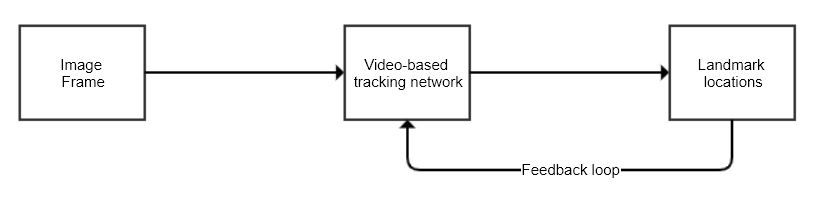
\includegraphics[scale=0.5]{generic_video_based}
\caption{Generic architecture of video based methods. Landmarks detected in the current frame are used as an initialization for the next frame}
\end{figure}

\section{Datasets}

The following table shows a multitude of datasets to train and evaluate face tracking models:


\begin{table}[htbp]
\caption{Datasets}
\begin{tabular}{|l|l|l|l|l|}
\hline
\textbf{Dataset} & \textbf{Description}                   & \textbf{Contains}                                                                                                                                 & \textbf{Wild?} & \textbf{Publicly available?} \\ \hline
300VW            & 300 videos in the wild                 & \begin{tabular}[c]{@{}l@{}}114 videos with 218,595 frames with 68\\  landmarks per frame\end{tabular}                                             & Yes            & Yes                          \\ \hline
AFLW             & Annotated Facial Landmarks in the Wild & \begin{tabular}[c]{@{}l@{}}Around 25k annotated face images with 21 \\ landmarks per image\end{tabular}                                           & Yes            & Yes                          \\ \hline
LFW              & Labeled Faces in the Wild              & \begin{tabular}[c]{@{}l@{}}13,233 images of 5749 people detected \\ and centered by Viola Jones face detector\end{tabular}                        & Yes            & Yes                          \\ \hline
Helen            & Helen facial feature dataset           & \begin{tabular}[c]{@{}l@{}}2000 training and 330 test images with \\ accurate consistent annotations of primary \\ facial components\end{tabular} & Yes            & Yes                          \\ \hline
LFPW             & Labeled Face Parts in the Wild         & \begin{tabular}[c]{@{}l@{}}1432 images with 29 landmarks on each \\ image\end{tabular}                                                            & Yes            & Yes                          \\ \hline
TF               & Talking Face                           & \begin{tabular}[c]{@{}l@{}}500 images of 5 videos with 68 landmarks \\ on each image\end{tabular}                                                 & No             & Yes                          \\ \hline
FM               & Face Movies                            & \begin{tabular}[c]{@{}l@{}}2150 images of 6 videos with 68 landmarks \\ on each image\end{tabular}                                                & Yes            & Yes                          \\ \hline
SynHead          & Synthetic dataset                      & 510,960 frames of 70 head motion tracks                                                                                                           & Yes            & Yes                          \\ \hline
BIWI             & Biwi kinect head pose database         & Over 15k frames of 20 people                                                                                                                      & Yes            & Yes                          \\ \hline
COFW             & Caltech Occluded Faces in the Wild     & \begin{tabular}[c]{@{}l@{}}1007 images with 29 manually annotated \\ landmarks on each image\end{tabular}                                         & Yes            & Yes                          \\ \hline
\end{tabular}
\end{table}

\section{Face Tracking Approaches}

\subsection{Recurrent Encoder-Decoder Network for Video-based Face Alignment (2017)}

This method leverages temporal information to predict facial landmarks in each frame. It uses recurrent learning at both spatial and temporal dimensions. At the temporal level, the features are separated into \textit{temporal-variant} features such as pose and expression, and \textit{temporal-invariant} features such as facial identity and recurrent learning is applied to the temporal-variant features. This feature disentangling has shown to achieve better generalization and more accurate results. Figure 2 shows the pipeline of recurrent encoder-decoder network \\

\begin{figure}
\copyrightbox[b]{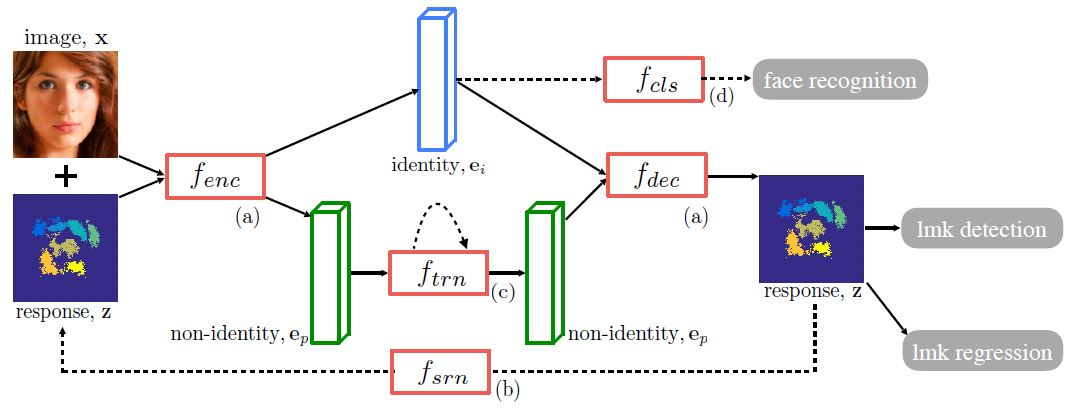
\includegraphics[scale=0.5]{rednet_architecture}}%
{Source: Xi Peng, Rogerio S. Feris, Xiaoyu Wang, Dimitris N. Metaxas. RED-Net: A Recurrent Encoder-Decoder Network for Video-based Face Alignment}
\caption{Overview of REDNet pipeline}
\end{figure}

The network consists of 4 modules -
\begin{itemize}
\item[(1)] \textbf{Encoder-Decoder}:-
The encoder encodes features from a single video frame into an intermediate low dimensional representation by performing a sequence of convolutions, pooling and batch normalization. The decoder upsamples the low dimensional representation and transforms it into a response map that contains facial landmarks.\\


\item[(2)] \textbf{Spatial recurrent learning}:-
The purpose is to find the exact location of landmarks in a coarse-to-fine manner by iteratively providing the previous prediction as feedback along with the video frame. This is carried out in 2 steps - \textit{Landmark detection} and \textit{Landmark Regression}. Landmark detection step locates 7 major facial components whereas landmark regression step refines predicted locations of all 68 landmark positions\\

\item[(3)] \textbf{Temporal recurrent learning}:-
This is proposed to model the temporal-variant factors such as pose and expression. The temporal variations in the temporal-invariant factors (non-identity code) are modeled using an LSTM unit consisting of 256 hidden neurons.
Trained using \textit{T} successive frames. Detection and regression tasks are performed frame by frame. The prediction loss is calculated at each time step. 
\\

\item[(4)] \textbf{Supervised identity disentangling}:-
Complete identity and non-identity factor disentangling cannot be guaranteed. More supervised information is needed to achieve better separation of the features. This module applies identity constraint to the identity code to further separate identity code from the non-identity code. Face recognition is applied to the identity code to classify the people present in the frames. \\
\end{itemize}

This model is trained on both image and video datasets with different configurations for different datasets. The datasets used are AFLW, LFW, Helen, LFPW, TF, FM and 300-VW

\subsection{Dynamic Facial Analysis using Recurrent Neural Networks (2017)}

This approach improvises on previous approaches for dynamic facial analysis which use Kalman filters or particle filters, inspired by the fact that RNNs and Bayesian filters are operationally very similar.
Bayesian filters need problem-specific designing. Given sufficient data, an RNN can be trained to do the same task and avoid problem-specific tracker engineering.
The model uses a synthetic dataset \textbf{SynHead} by NVIDIA for training to estimate head pose. The approach employs FC-RNN to exploit the generalization from a pre-trained CNN. It consists of CNN layers followed by recurrent layers as dense layers. RNN is more robust to occlusions and large head poses. Figure 3 shows the proposed end-to-end network for joint estimation and tracking. The CNN and RNN are trained together end-to-end.

\begin{figure}
\copyrightbox[b]{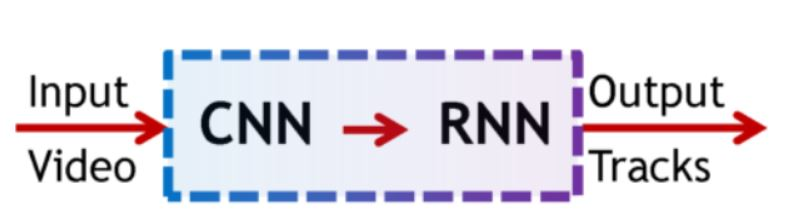
\includegraphics[scale=0.5]{cnn_rnn}}%
{Source: Jinwei Gu, Xiaodong Yang, Shalini De Mello, Jan Kautz. Dynamic Facial Analysis: From Bayesian Filters to Recurrent Neural Network}
\caption{Proposed end-to-end CNN RNN network}
\end{figure}


\subsection{Dual-Agent Deep Reinforcement Learning (2018)}

This approach exploits the fact that bounding box tracking and landmark detection are dependent. The accuracy of facial landmarks detected depends on how good the bounding box is. The architecture consists of a \textit{Tracking agent} and an \textit{Alignment agent} and \textit{communication channels} between the agents. The two agents are trained simultaneously to learn two conditional distributions. Figure 4 shows the proposed architecture. Bounding box adjustment and landmark regression are done simultaneously over many iterations.

\begin{figure}
\copyrightbox[b]{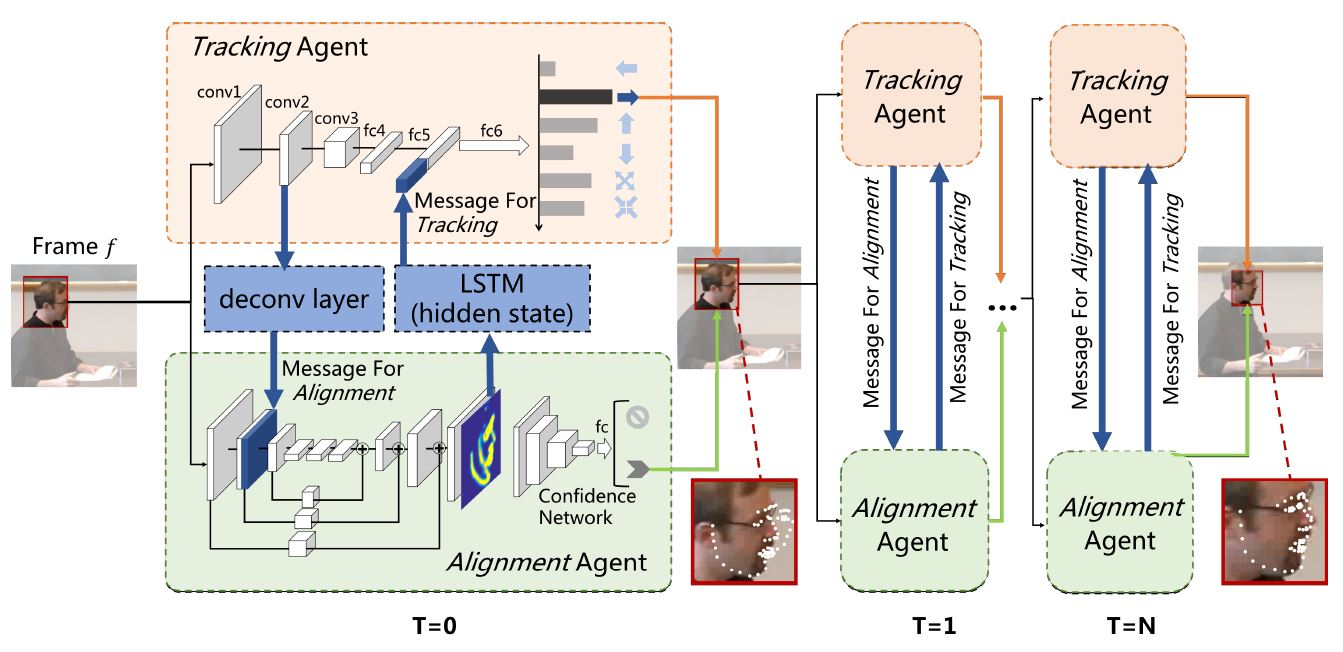
\includegraphics[scale=0.5]{DADRL}}%
{Source: Minghao Guo, Jiwen Lu, Jie Zhou. Dual-Agent Deep Reinforcement Learning for Deformable Face Tracking}
\caption{Proposed end-to-end CNN RNN network}
\end{figure}

\subsection{Two Stream Transformer Networks (2017)}

This approach aims to capture both spatial as well as temporal information. It proposes a two-stream deep learning method for video-based face alignment. The spatial stream aims to capture information on still frames. It is trained to transform image pixels to landmark positions directly on still frames. The temporal stream aims to capture temporal consistency information across successive frames. It is trained to encode all facial changes in the temporal dimension. It is followed by an RNN to model the sequential information over consecutive frames. Facial landmarks are determined by a weighted fusion of both spatial and temporal streams. Figure 5 shows the proposed architecture.

\begin{figure}
\copyrightbox[b]{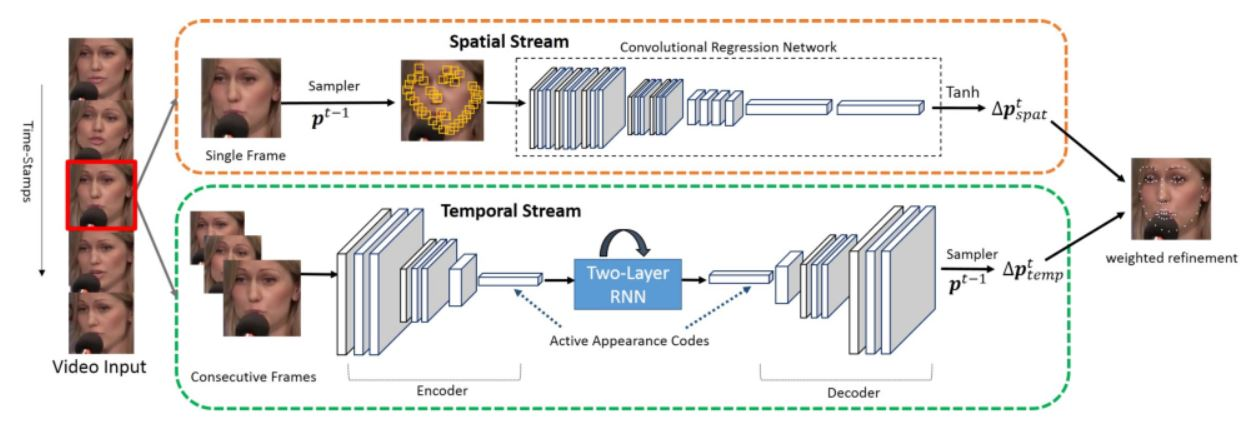
\includegraphics[scale=0.5]{TSTN}}%
{Source: Hao Liu, Senior Member, IEEE, Jianjiang Feng, Member, IEEE, Jie Zhou, Senior Member, IEEE. Two-Stream Transformer Networks for Video-based Face Alignment}
\caption{TSTN pipeline}
\end{figure}

\subsection{Face Alignment Recurrent Network (2017)}

This recurrent regression approach for landmark detection uses the LSTM model to exploit both spatial and temporal information. The predicted landmark location is used as a basis for estimation in the next stage (spatial) and used as a basis for estimation in the next frame (temporal).





\section{Performance Comparison}


\section{Discussion}


\section{Conclusion}


%

%
% ---- Bibliography ----
%
\bibliographystyle{plain}
\bibliography{bibexample}
%
\end{document}